\documentclass[11pt]{article}

\usepackage{acl}
\usepackage{times}
\usepackage{latexsym}
\usepackage{graphicx}
\usepackage{booktabs}
\usepackage{multirow}
\usepackage{amsmath}
\usepackage{amssymb}
\usepackage{url}
\usepackage{microtype}
\usepackage{xcolor}
\usepackage{pifont}
\newcommand{\cmark}{\ding{51}}
\newcommand{\xmark}{\ding{55}}

\title{TempoRAG-KG: Temporal Knowledge Graph-Augmented\\
Retrieval for Multi-Hop Question Answering\\
\large Progress Report}

\author{
  Supanut Kompayak \\
  st126055@ait.asia \\
  \textit{Asian Institute of Technology}
  \And
  Aphisit Jaemyaem \\
  st126130@ait.asia \\
  \textit{Asian Institute of Technology}
  \AND
  Dechathon Niamsa-ard \\
  st126235@ait.asia \\
  \textit{Asian Institute of Technology}
  \And
  Kaung Hein Htet \\
  st126477@ait.asia \\
  \textit{Asian Institute of Technology}
}

\begin{document}
\maketitle

% -------------------------------------------------------
% ABSTRACT
% -------------------------------------------------------
\begin{abstract}
We report mid-project progress on \textbf{TempoRAG-KG}, a retrieval-augmented
generation (RAG) system that couples a temporal knowledge graph with
chunk-level retrieval to answer multi-hop, time-sensitive questions. During
the first half of the project we piloted HotpotQA and MuSiQue as evaluation
corpora, but found that their Wikipedia-anchored factoids do not reliably
carry the kind of temporal structure our hypothesis targets. We therefore
pivoted to a corpus of 25 SEC 10-K filings (5 technology mega-caps $\times$ 5
fiscal years, 2019--2024), producing 7{,}467 item-level chunks and a
hand-vetted question bank of 129 items (50 home-grown + 79 multi-hop).
On this corpus we have completed two of four retrieval conditions across
7 LLMs spanning 3 providers. Our first key finding is that a temporal
year-mask applied on top of cosine retrieval (TimeFilter, L1) produces a
\textit{universal} positive lift over a vanilla baseline (L0), ranging from
+5.6\,\% to +24.7\,\% in token-F1. However, the hop=3 slice barely moves
(+0.007), which isolates the gap that our knowledge-graph conditions (L2, L3)
are designed to close. KG extraction over the full corpus is in progress at
the time of writing; L2 / L3 retrievers, ablations, and the final
interaction analysis remain as the closing phase of the project.
\end{abstract}

% -------------------------------------------------------
% 1. INTRODUCTION
% -------------------------------------------------------
\section{Introduction}
\label{sec:intro}

Retrieval-augmented generation \citep{lewis2020retrieval} has become a
standard recipe for question-answering over document corpora, but
off-the-shelf dense retrieval struggles when the \emph{same entity}
is described differently across time. A question such as ``did Microsoft's operating margin improve after
the Activision acquisition?'' requires the system to reason over facts
that are true in one fiscal year and false in another --- a property that
flat chunk similarity is blind to.

\paragraph{A discovery-driven pivot.}
Our original proposal planned to evaluate on HotpotQA
\citep{yang2018hotpotqa} and MuSiQue \citep{trivedi2022musique}. During
an EDA pass we inspected the temporal expressions present in those
benchmarks and found two problems. First, the vast majority of multi-hop
bridges are temporally static (``who was born in X?''), so even a perfect
year filter cannot demonstrate lift. Second, Wikipedia text drifts: the
``gold'' supporting sentence may have been edited after the QA pair was
written, which leaks noise into any retrieval-quality metric. This pushed
us to look for a corpus where (a) each document is stamped with a
machine-verifiable fiscal year, and (b) the same entity is described at
multiple, non-overlapping points in time. SEC 10-K filings satisfy both
criteria directly: each filing's fiscal-year metadata is authoritative,
and a 5-year window over 5 issuers gives 25 documents that repeatedly
re-describe the same entities.

\paragraph{What this report covers.}
This progress report documents (i) the motivation for the pivot, (ii) the
10-K corpus and QA set we assembled, (iii) the pipeline we have built so
far, and (iv) the first evaluation results from the L0 (vanilla cosine)
and L1 (TimeFilter) conditions across seven LLMs. The two remaining
conditions, L2 (KG$^{2}$RAG-style graph walk) and L3 (TempoRAG-KG with
temporal edges), depend on the running KG extraction and are discussed
as in-flight work in Section~\ref{sec:progress}.

\paragraph{Contributions to date.}
\begin{enumerate}
\itemsep 0pt \parskip 0pt
  \item A 7{,}467-chunk, item-level SEC 10-K corpus tailored to
    temporal multi-hop evaluation, with a 129-item hand-vetted QA set
    annotated for hop count and temporal scope.
  \item A reproducible retrieval + evaluation harness (cached embeddings,
    cached generations, bootstrap CIs) supporting 7 LLMs $\times$ 3
    providers on identical questions.
  \item Empirical evidence that a deterministic year-mask alone produces
    universal positive F1 lift, but leaves the hop=3 slice effectively
    flat --- motivating the KG conditions that constitute the remainder
    of the project.
\end{enumerate}

% -------------------------------------------------------
% 2. RELATED WORK
% -------------------------------------------------------
\section{Related Work}
\label{sec:related}

\paragraph{Graph-based RAG.}
Using a knowledge graph to guide retrieval is an active area
\citep{edge2024graphrag}; our work builds directly on KG$^{2}$RAG.
Zhu~et~al.\ propose augmenting chunk retrieval with a graph walk over
entity-linked seeds to widen the context available to the generator
\citep{zhu2025kg2rag}. We adopt this as our L2 condition. Crucially,
KG$^{2}$RAG's graph is untyped with respect to time: an edge either
exists or does not. Our L3 condition extends the same retrieval signal
with temporal validity intervals on each edge.

\paragraph{TempAgent and GoG.}
Several recent systems layer a planner over the graph to decide
\emph{which} edges to expand next \citep{tempagent2025,he2024gog}. Our
design differs: we do not plan, we simply mask the candidate pool by
fiscal year (L1) or by overlap of the question's year scope with each
edge's validity window (L3). This keeps the experiment interpretable ---
any lift we observe is attributable to the temporal signal, not to
emergent planner behaviour.

\paragraph{FinReflectKG-MultiHop.}
Kishore~et~al.\ recently released a multi-hop QA set over 10-K filings
derived from a KG-constrained generator \citep{finreflectkg2025}. We use
a subset of their questions (79 items) as an external anchor alongside
our own 50 home-grown questions, so that our evaluation does not rely
exclusively on questions we authored ourselves.

% -------------------------------------------------------
% 3. RESEARCH QUESTIONS
% -------------------------------------------------------
\section{Research Questions}
\label{sec:rqs}

The experimental design is a $2\times2$ factorial over the two
interventions the system combines: presence/absence of a \emph{temporal
filter} and presence/absence of a \emph{knowledge-graph walk}
(Table~\ref{tab:2x2}). The four cells correspond to the four pipeline
conditions introduced in Section~\ref{sec:pipeline}. All research
questions below are stated against this matrix so that each one maps
cleanly to a specific cell comparison.

\begin{table}[h]
\centering
\small
\setlength{\tabcolsep}{4pt}
\begin{tabular}{@{}lll@{}}
\toprule
            & No KG                   & \textbf{+ KG}            \\
\midrule
No Temporal & L0 Vanilla \cmark       & L2 KG$^{2}$RAG \xmark    \\
\textbf{+ Temporal} & L1 TimeFilter \cmark & L3 TempoRAG-KG \xmark    \\
\bottomrule
\end{tabular}
\caption{$2\times2$ experimental design. \cmark\ = complete at the time
of this report; \xmark\ = pending KG extraction.}
\label{tab:2x2}
\end{table}

\paragraph{RQ1 --- Where does KG$^{2}$RAG fail on temporal multi-hop QA?}
\textbf{IV:} graph walk on, temporal off (L2 cell, relative to L0).
\textbf{DV:} per-slice token-F1 (hop, scope). \textbf{H1:} KG$^{2}$RAG
improves over Vanilla on hop-$\geq$2 slices but leaves an identifiable
\emph{temporal} failure mode that a graph walk alone cannot close.
\emph{Pending KG extract.}

\paragraph{RQ2 --- Does TempoRAG-KG lift token-F1 over KG$^{2}$RAG?}
\textbf{IV:} temporal edges on / off with the KG held constant
(L3 vs L2). \textbf{DV:} token-F1 on the 129-item QA set and on the
hop-$\geq$2 slice. \textbf{H2:} L3 $>$ L2 with the largest gain on
slices where the question explicitly spans fiscal years
(\textit{inter\_year}, \textit{fiscal\_vs\_calendar}). \emph{Pending.}

\paragraph{RQ3 --- How accurate is the temporal KG extraction?}
\textbf{IV:} the extraction prompt (Appendix~\ref{app:extract}) applied
to each of the 7{,}467 chunks. \textbf{DV:} fraction of extracted triples
whose \texttt{valid\_from} / \texttt{valid\_to} intervals agree with the
source filing's fiscal-year metadata. \textbf{H3:} temporal-interval
accuracy is high enough that the L3 retriever's ceiling is bounded by
graph coverage (a design question), not by spurious intervals (a data
question). \emph{Measured once the full extract completes.}

\paragraph{RQ4 ($\star$) --- Can a small LM with temporal grounding
approach a large LM without it?}
\textbf{IV:} model scale crossed with retrieval condition (the seven
models in Table~\ref{tab:models} $\times$ L0--L3). \textbf{DV:} the
gap between the best small-open-model (llama-3.1-8B or gpt-oss-20B) at
L3 and the best large-closed-model (gpt-4o) at L0. \textbf{H4:} temporal
grounding substantively narrows this gap --- i.e.\ capability and
retrieval are partially substitutable for temporal QA. This is the
headline question for the project and the one our design is optimised
around.

\paragraph{Current state.} Section~\ref{sec:results} reports the
L0 vs L1 comparison, which is not by itself sufficient to answer any of
RQ1--RQ4 but does supply one necessary input: the size and uniformity
of the lift that a purely temporal signal, with no KG, can produce on
this corpus. The results are consistent with RQ4's hypothesis in the
directional sense (small models benefit at least as much as large
models from the temporal filter), but a definitive answer requires the
L2 and L3 cells.

% -------------------------------------------------------
% 4. METHODOLOGY
% -------------------------------------------------------
\section{Methodology}
\label{sec:method}

\subsection{Corpus}
\label{sec:corpus}
We downloaded 10-K filings directly from the SEC EDGAR API
(\texttt{data.sec.gov/submissions}) using a custom rate-limited
(5~req/s) downloader (\texttt{scripts/download\_10k.py}) and verified
each filing with its SHA-256 digest. The core evaluation corpus uses
the five technology mega-caps --- AAPL, MSFT, GOOGL, AMZN, META ---
across fiscal years 2019--2024 (25 filings). We segment each filing
into item-level chunks (Items~1, 1A, 7, 7A, 8) of approximately 1{,}000
tokens, producing 7{,}467 chunks. All chunks are embedded once with
\texttt{text-embedding-3-small} and cached
(total embedding spend: approximately \$0.07).

\subsection{QA Set}
\label{sec:qa}
Our 129-item QA set is assembled from two sources:
\begin{itemize}
\itemsep 0pt \parskip 0pt
  \item 50 \textit{home-grown} questions authored by the team and
    cross-reviewed for factual correctness against the underlying
    filings.
  \item 79 questions drawn from \textsc{FinReflectKG-MultiHop}, filtered
    to those whose gold answer span is present in our 25-filing
    corpus.
\end{itemize}
Every question is annotated with a hop count and a scope label
(\textit{intra}, \textit{inter\_year}, \textit{cross\_company},
\textit{fiscal\_vs\_calendar}, \textit{forward\_looking}).
Table~\ref{tab:qa-scope} summarises the scope distribution for the
home-grown half; the multi-hop half is scope-mixed and dominated by
$hop=2$ items ($n=104$).

\begin{table}[h]
\centering
\small
\begin{tabular}{lr}
\toprule
Scope & Count \\
\midrule
cross\_company       & 18 \\
inter\_year          & 15 \\
intra                & 10 \\
fiscal\_vs\_calendar &  5 \\
forward\_looking     &  2 \\
\midrule
\textbf{Total (home-grown)} & \textbf{50} \\
\bottomrule
\end{tabular}
\caption{Scope distribution of the 50 home-grown questions.
Scope is an orthogonal axis to hop count: a \textit{cross\_company}
question may be hop~2 or hop~3 depending on how many filings are
required to answer it.}
\label{tab:qa-scope}
\end{table}

\subsection{Pipeline}
\label{sec:pipeline}
Figure~\ref{fig:pipeline} shows the full pipeline: 25 filings are
chunked, embedded once, and fed to four retrieval branches that share
a single answer-generation stage. The two completed branches are:

\begin{itemize}
\itemsep 0pt \parskip 0pt
  \item \textbf{L0 Vanilla} --- top-$k$ cosine retrieval over all
    7{,}467 chunks (\texttt{retrieve} in \texttt{src/retrieval.py}).
  \item \textbf{L1 TimeFilter} --- same retrieval, but scores for
    chunks whose fiscal year is not in the question's year set are
    masked to $-\infty$ (\texttt{retrieve\_with\_year\_filter} in
    the same module).
\end{itemize}
If the masked pool contains fewer than $k$ chunks, we fall back to the
unfiltered pool to avoid empty contexts. The two pending branches
(L2, L3) share the same generator and prompt and differ only in how
the candidate pool is assembled.

\begin{figure}[t]
\centering
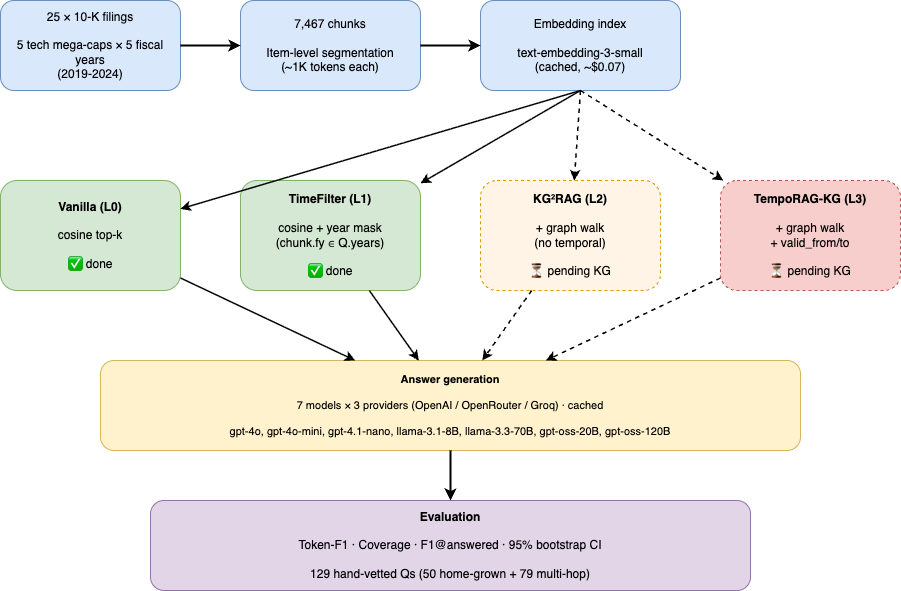
\includegraphics[width=\linewidth]{../docs/progress_report/pipeline.png}
\caption{End-to-end pipeline. Blue: corpus preparation (done). Green:
completed retrieval branches (L0, L1). Orange/red dashed: pending
retrieval branches (L2, L3). Yellow: shared answer-generation stage.
Purple: evaluation.}
\label{fig:pipeline}
\end{figure}

\subsection{Metrics}
\label{sec:metrics}
We report \textbf{Token-F1} with SQuAD-style normalisation,
\textbf{Coverage} (the fraction of rows where the model attempted an
answer rather than refusing), and \textbf{F1@answered} (token-F1
restricted to the answered subset). All intervals are 95\,\%
non-parametric bootstrap CIs with $n=1000$ and a fixed seed (the
implementation is \texttt{src/eval.py:aggregate} and
\texttt{src/eval.py:bootstrap\_ci}). A refusal or empty string is
detected by the \texttt{is\_idk} regex in the same module and counted
as not-answered rather than as a wrong answer.

\subsection{Models}
\label{sec:models}
We run the same 129 questions through seven LLMs spanning three
providers so that any finding generalises across both scale and
vendor (Table~\ref{tab:models}).

\begin{table}[h]
\centering
\small
\begin{tabular}{lll}
\toprule
Model & Provider & Role \\
\midrule
gpt-4o              & OpenAI     & large, closed \\
gpt-4o-mini         & OpenAI     & mid, closed   \\
gpt-4.1-nano        & OpenAI     & small, closed \\
llama-3.1-8B        & Groq       & small, open   \\
llama-3.3-70B       & Groq       & large, open   \\
gpt-oss-20B         & OpenRouter & small, open   \\
gpt-oss-120B        & OpenRouter & large, open   \\
\bottomrule
\end{tabular}
\caption{The seven LLMs used as answer generators. All receive the
same retrieved context and the same prompt; only the model identity
varies.}
\label{tab:models}
\end{table}

\paragraph{Cost and caching.}
Each question $\times$ model $\times$ condition produces exactly one
generation, which is written to an on-disk cache keyed by prompt and
generation parameters; subsequent runs are free. The open-model rows
(llama-3.1-8B, llama-3.3-70B on Groq; gpt-oss-20B/120B on OpenRouter)
use free-tier endpoints; the three OpenAI models together produced
$\approx1{,}800$ cached generations for the L0 and L1 sweeps at a
total spend well under the project's \$20 budget. Cumulative
generation wall-clock across all 7 models is $\approx 2.2$\,hours.

% -------------------------------------------------------
% 5. RESULTS
% -------------------------------------------------------
\section{Results}
\label{sec:results}

This section reports the state of the evaluation at the time of
writing. Only the L0 and L1 conditions are complete; L2 and L3 rows
will be added once the KG extraction finishes and the L2/L3
retrievers are implemented.

\subsection{Overall}
\label{sec:r-overall}
Across all seven LLMs, the L1 year-mask strictly dominates the L0
vanilla baseline in token-F1 (Table~\ref{tab:overall}). The lift
ranges from +5.6\,\% (gpt-oss-120b) to +24.7\,\% (llama-3.1-8B), and
coverage also rises under L1, confirming that the mask is not simply
trading off retrieval precision for refusal rate.

\paragraph{Retrieval, not answer quality, is the bottleneck.}
Comparing L0 and L1 on the two sub-metrics makes this more precise.
L1 coverage rises by +3.1\,pp (gpt-oss-120b) to +10.1\,pp
(llama-3.3-70B) --- i.e.\ the mask causes the retrieved context to
contain an answerable span more often. But F1@answered --- the
token-F1 \emph{conditional} on the model having produced a non-refusal
--- barely moves between L0 and L1 (for example, gpt-4o goes from
0.385 to 0.391, gpt-4o-mini from 0.396 to 0.395). This pattern tells
us that, at current retrieval quality, each model's answer-writing
ability is already close to ceiling on whatever evidence it is given;
the further F1 lifts we are chasing must come from better retrieval
(KG walk, temporal edges), not from a larger generator.

\begin{table*}[t]
\centering
\small
\setlength{\tabcolsep}{4pt}
\begin{tabular}{l cc cc r c c}
\toprule
 & \multicolumn{2}{c}{L0 token-F1} & \multicolumn{2}{c}{L1 token-F1} & $\Delta\,\%$ & L1 Coverage & L1 F1@ans \\
\cmidrule(lr){2-3}\cmidrule(lr){4-5}
Model          & mean  & 95\%\,CI         & mean  & 95\%\,CI         &           &         &                      \\
\midrule
gpt-4.1-nano   & 0.229 & [0.194,\,0.270]  & 0.258 & [0.221,\,0.296]  & +12.7     & 70.5\%  & 0.366 [0.333,\,0.398] \\
gpt-4o         & 0.183 & [0.141,\,0.223]  & 0.221 & [0.184,\,0.264]  & +20.9     & 56.6\%  & 0.391 [0.348,\,0.432] \\
gpt-4o-mini    & 0.230 & [0.193,\,0.274]  & 0.248 & [0.206,\,0.290]  & \phantom{0}+7.8  & 62.8\% & 0.395 [0.357,\,0.435] \\
gpt-oss-20B    & 0.120 & [0.088,\,0.159]  & 0.145 & [0.110,\,0.184]  & +21.0     & 42.6\%  & 0.336 [0.279,\,0.391] \\
gpt-oss-120B   & 0.131 & [0.094,\,0.172]  & 0.138 & [0.103,\,0.181]  & \phantom{0}+5.6  & 38.8\% & 0.356 [0.296,\,0.418] \\
llama-3.1-8B   & 0.145 & [0.114,\,0.180]  & 0.180 & [0.147,\,0.216]  & +24.7     & 57.4\%  & 0.314 [0.276,\,0.355] \\
llama-3.3-70B  & 0.145 & [0.112,\,0.181]  & 0.179 & [0.144,\,0.215]  & +23.7     & 53.5\%  & 0.335 [0.294,\,0.373] \\
\bottomrule
\end{tabular}
\caption{Per-model token-F1 under L0 (vanilla cosine) and L1
(TimeFilter), with 95\,\% non-parametric bootstrap CIs ($n=1000$,
fixed seed). Relative lift, L1 coverage, and L1 F1@answered (with CI)
are shown on the right. The L1 mean is above the L0 mean for every
model; no L1--L0 delta flips sign inside its CI. L2 and L3 rows will
be added when those conditions complete.}
\label{tab:overall}
\end{table*}

\subsection{By hop count}
\label{sec:r-hop}
To see whether the year-mask alone is enough to handle multi-hop
questions, we slice by hop count for a representative small model
(\texttt{gpt-4.1-nano}, Table~\ref{tab:by-hop}). Two things stand
out. First, the hop=2 slice (the bulk of the QA set) improves by
+0.048 F1. Second --- and this is the main motivating observation
for the KG conditions --- the hop=3 slice moves by only +0.007,
i.e.\ the temporal signal on its own is effectively blind to the
genuinely multi-hop cases. This is the gap the L2 / L3 graph walk
is designed to close.

\begin{table}[h]
\centering
\small
\begin{tabular}{lr rr r}
\toprule
Hop & $n$ & L0    & L1    & $\Delta$ \\
\midrule
1   &  10 & 0.337 & 0.206 & $-$0.131 \\
2   & 104 & 0.234 & 0.281 & $+$0.048 \\
3   &  15 & 0.123 & 0.131 & $+$0.007 \\
\bottomrule
\end{tabular}
\caption{gpt-4.1-nano token-F1 by hop count.
The hop=1 regression is a known artefact: some hop=1 questions carry
a year label that is tighter than the span the filing actually
reports the answer in, so the hard mask removes the relevant chunk.
A softer temporal weighting is a natural mitigation but is outside
the scope of this report.}
\label{tab:by-hop}
\end{table}

\subsection{By temporal scope}
\label{sec:r-scope}
Table~\ref{tab:by-scope} stratifies the same gpt-4.1-nano run by the
scope label. The mask delivers its largest lift exactly where a year
mask \emph{should} help: on \textit{inter\_year} questions that span
multiple fiscal years ($+0.055$, $n=53$) and on \textit{cross\_company}
questions that still pin a year ($+0.051$, $n=24$). Two slices where
the mask cannot help are also visible. On \textit{intra} (same-year)
questions the mask is essentially a no-op ($\Delta=-0.001$, $n=45$):
the question and all candidate chunks already share one year, so
removing other years changes nothing. On \textit{fiscal\_vs\_calendar}
($n=5$) the mask actually regresses by $-0.079$, an expected
failure mode: a question of the form ``in Q3 2022\ldots'' has a
calendar-year stamp, but the answer lives in a filing stamped with a
fiscal year that may differ, and the hard mask removes the correct
filing. The sample is small ($n=5$) but the direction is the one we
predicted in Section~\ref{sec:rqs}.

\begin{table}[h]
\centering
\small
\begin{tabular}{lr rr r}
\toprule
Scope & $n$ & L0    & L1    & $\Delta$ \\
\midrule
inter\_year          & 53 & 0.220 & 0.276 & $+$0.055 \\
cross\_company       & 24 & 0.264 & 0.315 & $+$0.051 \\
forward\_looking     &  2 & 0.138 & 0.157 & $+$0.019 \\
intra                & 45 & 0.216 & 0.216 & $-$0.001 \\
fiscal\_vs\_calendar &  5 & 0.301 & 0.222 & $-$0.079 \\
\bottomrule
\end{tabular}
\caption{gpt-4.1-nano token-F1 by scope.
\textit{forward\_looking} ($n=2$) is not statistically meaningful and
is included only for completeness; the \textit{fiscal\_vs\_calendar}
regression is discussed in the text.}
\label{tab:by-scope}
\end{table}

% -------------------------------------------------------
% 6. PROGRESS SUMMARY
% -------------------------------------------------------
\section{Progress Summary}
\label{sec:progress}

\paragraph{Completed.}
Corpus preparation (25 filings, 7{,}467 chunks, cached embeddings),
QA-set construction (129 items, hop/scope annotated), retrieval
harness (L0, L1), evaluation harness (Token-F1, Coverage,
F1@answered, bootstrap CI), answer-generation cache across 7
models $\times$ 3 providers, and the progress-report slide deck.

\paragraph{In flight.}
KG extraction over the full corpus is currently running. Each
chunk is passed through a structured-extraction prompt that yields
typed triples with explicit \texttt{valid\_from} / \texttt{valid\_to}
intervals; this is the input substrate for both the L2 and L3
conditions.

\paragraph{Remaining work.}
A light filter pass on the extracted triples (drop trivially-true
relations, fix the comparative-value extraction bug); implementation
of the L2 (KG$^{2}$RAG-style) and L3 (TempoRAG-KG) retrievers;
identical 7-model sweeps for L2 and L3; the interaction analysis
required by RQ3; and the write-up.

\subsection{Limitations at this stage}
\label{sec:limits}
Four threats to validity deserve to be named explicitly before the
final report. \textbf{(i)}~The 129-item QA set is hand-vetted and
internally consistent but small; individual scope cells (especially
\textit{forward\_looking}, $n=2$, and \textit{fiscal\_vs\_calendar},
$n=5$) have too few items to support confident sub-claims on their
own. \textbf{(ii)}~The current results cover only the L0/L1 axis of
the $2\times2$ design; any claim about the KG contribution or about
the interaction between KG and temporal signal is \emph{not} supported
by this report. \textbf{(iii)}~L1 uses a \emph{hard} year mask: the
regression on \textit{fiscal\_vs\_calendar} (Table~\ref{tab:by-scope})
is a direct consequence of that design choice, and a softer
temporal weighting may recover that slice. \textbf{(iv)}~The corpus
is 25 filings from five issuers in one sector; findings should not
be extrapolated to financial QA in general without further
evaluation.

% -------------------------------------------------------
% 7. CONCLUSION
% -------------------------------------------------------
\section{Conclusion}
\label{sec:conclusion}

The evidence we have at the time of this report is narrow but clear:
on a 10-K corpus where every document carries an authoritative
fiscal-year label, a deterministic year-mask applied on top of a
cosine retriever raises token-F1 for every one of the seven LLMs we
tested, with no observed reversals. The same experiment also shows
that this temporal signal, on its own, essentially does not help on
the hop=3 slice. We read this as a clean separation of the two
effects our system is designed to combine: the L1 result establishes
that temporal grounding carries measurable signal on this corpus, and
it leaves the multi-hop gap open for the KG conditions to address.
Importantly, the L1 lift is as large for the two small open models
(llama-3.1-8B, gpt-oss-20B) as it is for the large closed models,
which is a directional signal in favour of RQ4 (Section~\ref{sec:rqs}).
The headline test --- whether a small LM at L3 approaches a large LM
at L0 --- remains the next and decisive milestone for the project.

% -------------------------------------------------------
% BIBLIOGRAPHY
% -------------------------------------------------------
\bibliography{references}

% -------------------------------------------------------
% APPENDIX
% -------------------------------------------------------
\appendix

\section{Extraction Prompt (v1)}
\label{app:extract}
See \texttt{prompts/extract\_v1.txt} in the repository. A verbatim
copy will be included in the final report.

\section{Answer Prompt}
\label{app:answer}
See \texttt{prompts/answer\_v1.txt}. The prompt is deliberately
minimal: it supplies the retrieved chunks, the question, and an
instruction to refuse if the answer is not present in the context.
Refusal phrasing is what the \texttt{is\_idk} regex in
\texttt{src/eval.py} is tuned to recognise.

\section{Scope Taxonomy}
\label{app:scope}
\begin{description}
\itemsep 0pt \parskip 0pt
\item[intra] Answer is contained within a single (filing, item) pair.
\item[inter\_year] Answer requires comparing two or more fiscal years
  of the same issuer.
\item[cross\_company] Answer requires comparing two or more issuers,
  possibly in a single year.
\item[fiscal\_vs\_calendar] Question references a calendar-year event
  (``Q3 2022'') that must be mapped onto the issuer's fiscal year.
\item[forward\_looking] Answer is a projection or guidance statement
  rather than a realised value.
\end{description}

\end{document}
